\section{CNN for Twitter sentiment}

\begin{figure}[htb]
\centering
  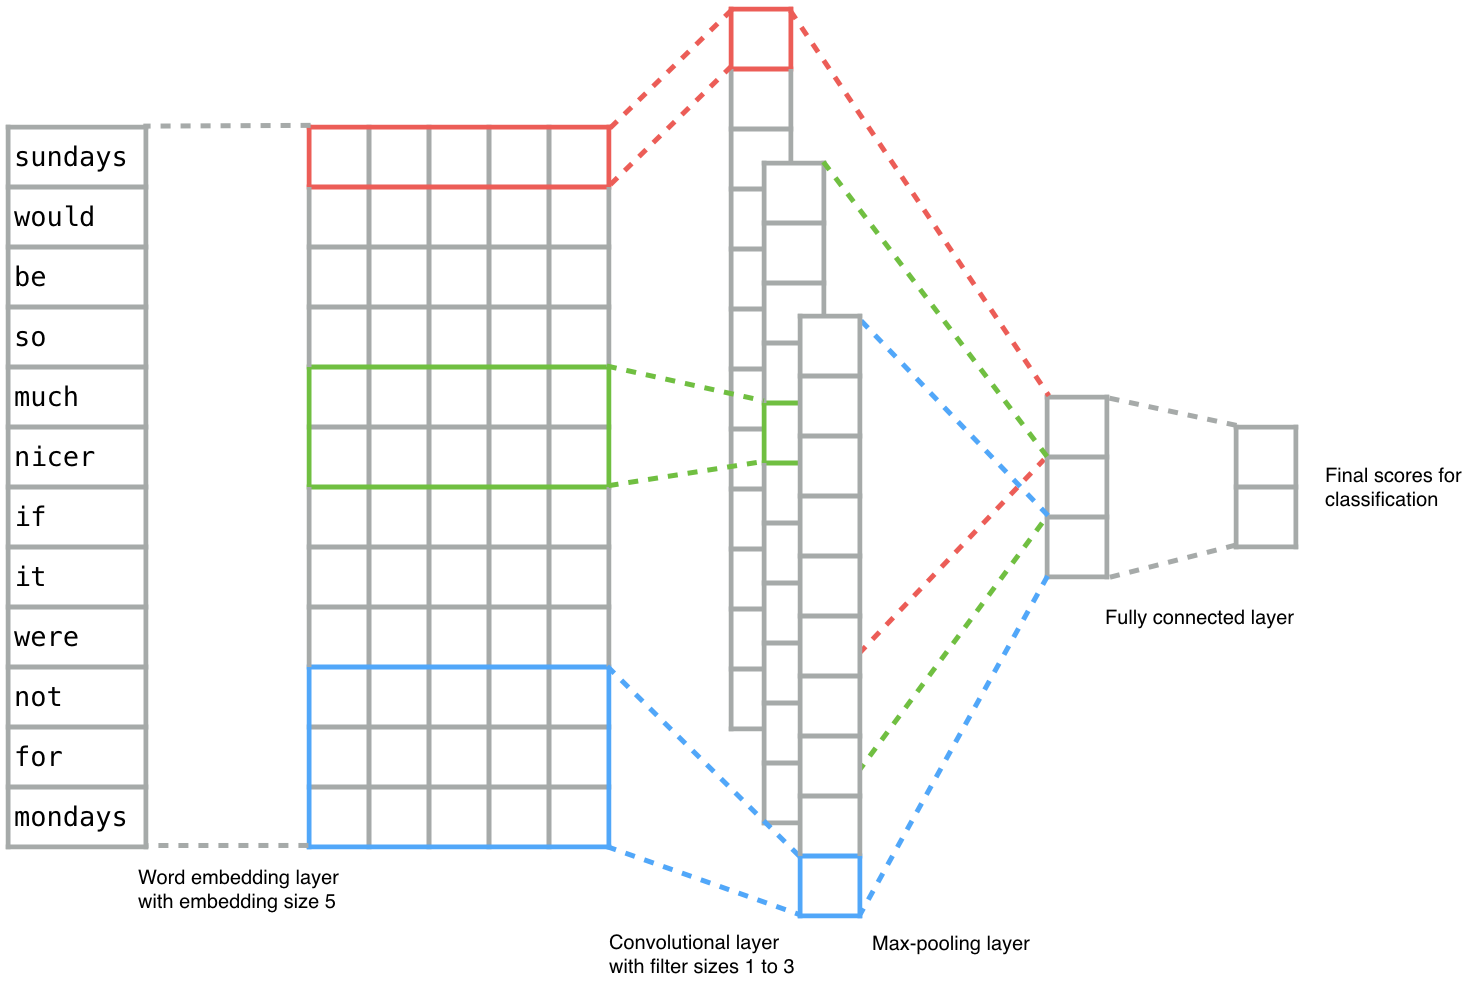
\includegraphics[width=0.8\linewidth]{figure/cnn.png}
  \caption{Structure of CNN}\label{fig.cnn}
\end{figure}

\subsection{Network structure}

The structure of the CNN used in our term project is shown in Figure \ref{fig.cnn}. It is a simplification of the model used in \cite{kim2014}. Although this model has a minimalist design, it has most of the typical layers of a text-mining CNN: word embedding layer, convolutional layer, max-pooling layer, and fully-connected layer.

The first layer is the word embeddings, which is encoded as a weight matrix that is used as a lookup table. Each row of the weight matrix is a vector of size $k$ represents a unique word in the vocabulary. Given a sentence of length $n$, padded if necessary, each word is replaced by its corresponding vector and the sentence is converted to an output matrix that is a concatenation of all the embeddings. This output matrix is represented as
$$
\textbf{x}_{1:n} = \textbf{x}_1 \oplus \textbf{x}_2 \oplus \ldots \oplus \textbf{x}_n
$$
where $\textbf{x}_i \in \mathbb{R}^k$ is the embedding of the $i$-th word in the sentence, and $\textbf{x}_{i:ij} \in \mathbb{R}^{kj}$ is used to denote the sub-matrix from the $i$-th word to the $j$-th word.

The second layer is the convolutional layer. Given a window size $h$, this layer is encoded by a {\em filter} $\textbf{w} \in \mathbb{R}^{hk}$. When this filter is applied to the $h$-gram $\textbf{x}_{i:i+h-1}$ of the input sentence, a feature $c_i$ is generated by
$$
c_i = f(\textbf{w} \cdot \textbf{x}_{i:i+h-1} + b)
$$
where $b \in \mathbb{R}$ is bias and $f$ is the activation function such as rectifier. The filter slides over all the possible $h$-grams of the input sentence to produce a feature map
$$
\textbf{c} = (c_1, c_2, \ldots, c_{n-h+1})
$$ 
for $\textbf{c} \in \mathbb{R}^{n-h+1}$.

The next layer is the max-pooling layer. It is applied to the feature map produced by the convolutional layer to produce a single feature $\hat{c} = \text{max}(\textbf{c})$. Taking the maximum essentially picks the most important feature in the feature map, which is an effective way to deal with variable sentence length, because the special word for padding has 0s in all the dimensions in its word embedding. 

The last layer is a fully-connected layer. The $\hat{c}$ is the selected feature by a {\em single} filter, there're a number of filters with different window sizes. All the selected features from these filters are the input for this fully-connected layer, which uses softmax function to calculate the score for each class. 

\subsection{Regularization}

The purpose of regularization is to prevent overfitting or co-adaptation. Unlike \cite{kim2014}, only dropout is used to prevent co-adaptation, because according to \cite{zhang2015} the L2-norm constraint used in \cite{kim2014} generally has little effect on the end result, and we want to keep the network as simple as possible. The dropout is applied to the fully-connected layer of the CNN. It works by randomly setting a proportion $p$ of hidden units to 0 during learning. During testing, the dropout is disabled and the learnt weights are scaled down by $p$.
